
\pgfplotsset{
%        compat=newest,  % <-- does not work; don't know why
        compat=1.13,     % <-- works as expected
    }
  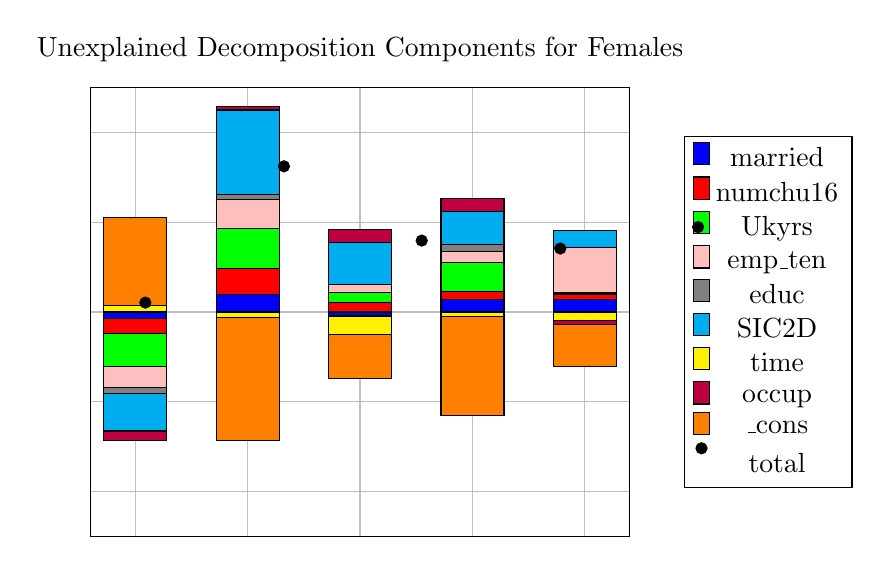
\begin{tikzpicture}
  %\node [align=center, font=\small, rotate=45,text width=2.15cm, inner sep=0.25cm] at (1, 1) {\textsc{year 1}};
  \begin{axis}[
    title={Unexplained Decomposition Components for Females},
    ybar stacked,
    ymax=0.5,
    ymin=-0.5,
    ymajorgrids = true,
    xmajorgrids = true,
    bar width=8mm,
    %xtick={1,2,3,4,5},
    %xticklabels={White, Black, Chinese, Asian, Mixed}
    symbolic x coords={White, Black, Chinese, Asian, Mixed},
    xtick=data,
    nodes near coords align={anchor=north},%Move values in bar
    every node near coord/.style={},
    legend style={at={(1.1,0.5)},anchor=west}
  ]
    %married
    \addplot [fill=blue] coordinates {
({White},-0.0154189)
({Black},0.0384454)
({Chinese},-0.0081768)
({Asian},0.0275639)
({Mixed},0.0288585)
};
    %numchu16
    \addplot [fill=red] coordinates {
({White},-0.0322832)
({Black},0.0592466)
({Chinese},0.021822)
({Asian},0.0186987)
({Mixed},0.0114051)
};
    %UKyrs
    \addplot [fill=green] coordinates {
({White},-0.0728362)
({Black},0.0883377)
({Chinese},0.0222342)
({Asian},0.064831)
({Mixed},0.0042565)
};

    %empten
    \addplot [fill=pink] coordinates {
({White},-0.0468162)
({Black},0.0641824)
({Chinese},0.017631)
({Asian},0.0243557)
({Mixed},0.0994206)
};
    %educ
    \addplot [fill=gray] coordinates {
({White},-0.0138101)
({Black},0.0111162)
({Chinese},-0.0027288)
({Asian},0.0147731)
({Mixed},-0.0008352)
};
    %SIC2D
    \addplot [fill=cyan] coordinates {
({White},-0.0841363)
({Black},0.1893483)
({Chinese},0.0938175)
({Asian},0.0734189)
({Mixed},0.0382063)
};
    %time
    \addplot [fill=yellow] coordinates {
({White},0.0139219)
({Black},-0.0124683)
({Chinese},-0.0390324)
({Asian},-0.0090862)
({Mixed},-0.0170767)
};
    %occup
    \addplot [fill=purple] coordinates {
({White},-0.0214268)
({Black},0.007055)
({Chinese},0.0285606)
({Asian},0.0290667)
({Mixed},-0.0090312)
};
    %_cons
    \addplot [fill=orange] coordinates {
({White},0.1965995)
({Black},-0.2741921)
({Chinese},-0.0978135)
({Asian},-0.221703)
({Mixed},-0.0942533)
};
\addplot [only marks,mark=*,mark size=2pt,black,
         nodes near coords = \rotatebox{90}{{\pgfmathprintnumber[fixed zerofill,
                                    precision=2]{\pgfplotspointmeta}}},
        nodes near coords align={vertical},
        point meta=y,
        every node near coord/.append style={font=\small, yshift=0.25mm},] coordinates {({Mixed},-1)};
%\begin{comment}
%\end{comment}
%\filldraw[black] (0,0) circle (2pt) node[anchor=west] {Intersection point};
  \legend{married, numchu16, Ukyrs, emp\_ten, educ, SIC2D, time, occup, \_cons, total}
  \end{axis}
  
  \begin{axis}[
    nodes near coords align={anchor=north},%Move values in bar
    every node near coord/.style={},
    xtick=data,
    ymax=0.3,
    ymin=-0.3,
    xmax=0,
    xmin=5,
]
\pgfplotsset{ticks=none}
\addplot[only marks,mark=*,mark size=3pt,black,
         nodes near coords = \rotatebox{90}{{\pgfmathprintnumber[fixed zerofill,
                                    precision=2]{\pgfplotspointmeta}}},
        nodes near coords align={vertical},
        point meta=y,
        every node near coord/.append style={font=\small, yshift=0.25mm},
        ]  coordinates {
    (1,0.1) (2,-0.1) (3,1)
};
\end{axis}
\filldraw[black] (0.7,2.9665559) circle (2pt) node[anchor=west] {};
\filldraw[black] (2.46,4.6974984) circle (2pt) node[anchor=west] {};
\filldraw[black] (4.21,3.7541959) circle (2pt) node[anchor=west] {};
\filldraw[black] (5.97,3.6534316) circle (2pt) node[anchor=west] {};
\filldraw[black] (7.72,3.9266542) circle (2pt) node[anchor=west] {};
  \end{tikzpicture}
